\section{Alberi Binari di Ricerca}
\paragraph{Albero binario:} struttura di dati ad albero composta da nodi, ognuno dei quali ha al massimo due figli, chiamati nodo destro e nodo sinistro. L'albero inizia con un singolo nodo, noto come radice. \\~\\

Matematicamente:
\begin{itemize}
    \item nodi $x$ ed elemento/valore/chiave $x.key$
    \item operazioni hanno costo $O(h)$ quando non bilanciato, $O(\log(n))$ se bilanciato
\end{itemize}

\paragraph{Definizione induttiva:}
\begin{itemize}
    \item $\varnothing$ è un albero
    \item se $r$ è un nodo, $T_1$ e $T_2$ alberi $\Rightarrow r(T_1,T_2)$ è un albero
    \item ogni nodo $x$ ha i seguenti campi:
    \begin{itemize}
        \item $x.p$
        \item $x.key$
        \item $x.left$
        \item $x.right$
    \end{itemize}
\end{itemize}

\paragraph{Operazioni possibili:}
\begin{itemize}
    \item Visita simmetrica (InOrder)
    \item Ricerca (Search)
    \item Ricerca di min e max
    \item Successore
    \item Inserimento
    \item Cancellazione
\end{itemize}

\subsection{Visita simmetrica (InOrder)}
Elencare gli elementi del sottoalbero radicato in un nodo $x$ in ordine di chiave crescente.
\begin{mdframed}
\begin{lstlisting}[language=C]
IN-ORDER(x)
1   if x != NULL
2       IN-ORDER(x.left)
3       print(x)
4       IN-ORDER(x.right)
\end{lstlisting}
\end{mdframed}
La complessità di tale operazione è lineare, dato da una visita di tutto l'albero.
\begin{equation*}
    T(n) = \begin{cases}
        c \qquad(n=0)\\
        T(k) + T(n-k-1) + d \qquad(n>0, k<n)
    \end{cases}
\end{equation*}
Stima di complessità: $T(n) = (c+d)n + c$

\newpage
\subsection{Ricerca (Search)}
Data $k$ chiave, cerca nel sottoalbero radicato nel nodo $x$ un nodo con chiave $k$.
\begin{mdframed}
\begin{lstlisting}[language=C]
SEARCH(x,k)
1   if (x == NULL) or (x.key == k)
2       return x
3   else if (k < x.key)
4       return SEARCH(x.left,k)
5   else
6       return SEARCH(x.right,k)
\end{lstlisting}
\end{mdframed}
La complessità, nel caso peggiore, è la ricerca che continua fino ad una foglia ed il cammino radice-foglia è quello massimo. Complessità: $O(h)$.
\begin{mdframed}
\begin{lstlisting}[language=C]
SEARCH(x,k)
1   while (x != NULL) and (x.key != k)
2       if (k < x.key)
3           x = x.left
4       else
5           x = x.right
6   return x
\end{lstlisting}
\end{mdframed}
Se dobbiamo esaminare tutto l'albero, nel caso peggiore avremo una complessità $\Theta(n)$ sulla base di una relazione di ricorrenza $T(n) = c + T(k) + T(n-k-1)$. 

\subsection{Ricerca di min e max}
Ricerca continuando ad andare verso sx oppure continuando ad andare verso dx. Per entrambi, la complessità è data dall'altezza dell'albero, in generale $O(h)$.
\begin{multicols}{2}
\begin{mdframed}
\begin{lstlisting}[language=C]
MIN(T)
1   x = T.root
2   if x == NULL
3       return NULL
4   else
5       while x.left != NULL
6           x = x.left
7       return x
\end{lstlisting}
\end{mdframed}
\begin{mdframed}
\begin{lstlisting}[language=C]
MAX(T)
1   x = T.root
2   if x == NULL
3       return NULL
4   else
5       while x.right != NULL
6           x = x.right
7       return x
\end{lstlisting}
\end{mdframed}
\end{multicols}

\subsection{Successore}
Si intende il nodo elencato dopo un nodo $x$ passato come parametro in una visita simmetrica. \\~\\
Dato $x \in ABR$:
\begin{itemize}
    \item minimo tra i nodi più grandi di $x$
    \item nodo che segue $x$ in una visita \verb|InOrder|
    \item se $x$ ha sottoalbero dx non vuoto $\Rightarrow$ il successore è $\min(x.right)$
    \item se $x$ non ha sottoalbero dx $\Rightarrow$ il successore è ilpiù vicino antenato di $x$ è nel sottoalbero sx
\end{itemize}
\begin{mdframed}
\begin{lstlisting}[language=C]
SUCCESSOR(x)
1   if x.right != NULL
2       return MIN(x.right)
3   else
4       y = x.p
5       while (y != NULL) and (x == y.right)
6           x = y
7           y = y.p
8       return y
\end{lstlisting}
\end{mdframed}
Complessità: $O(h)$.

\subsection{Inserimento}
La funzione \verb|Insert| viene utilizzata per aggiungere un nuovo elemento in un albero di ricerca binario in una posizione appropriata. \\~\\
La funzione \verb|Insert| deve essere progettata in modo tale da non violare la proprietà dell'albero di ricerca binario a ogni valore.
\begin{enumerate}
    \item Allocare la memoria per l'albero.
    \item Impostare la parte dei dati sul valore e impostare il puntatore sx e dx dell'albero su NULL.
    \item Se l'elemento da inserire sarà il primo elemento dell'albero, i puntatori sx e dx di questo nodo punteranno a NULL.
    \item In caso contrario, controlla se l'elemento è inferiore all'elemento radice dell'albero. 
    \item Se è vero, esegue ricorsivamente l'operazione con la sx della radice.
    \item Se è falso, allora si esegue questa operazione ricorsivamente con il sottoalbero dx della radice.
\end{enumerate}
\begin{mdframed}
\begin{lstlisting}[language=C]
INSERT(T,z)
1   x = T.root
2   y = NULL
3   while x != NULL
4       y = x
5       if z.key < x.key
6           x = x.left
7       else
8           x = x.right
9   z.p = y
10  if y == NULL
11      T.root = z
12  else
13      if z.key < y.key
14          y.left = z
15      else
16          y.right = z
\end{lstlisting}
\end{mdframed}
Complessità: $O(h)$.

\subsection{Cancellazione}
Distinguiamo due casi:
\begin{itemize}
    \item $z$ ha al più un figlio
    \item $z$ ha due figli $\Rightarrow$ pericoloso: rischio che si copino i dati di $y$ in $z$.
\end{itemize}
Creiamo una funzione \verb|Transplant|, che cerca di sostituire il nodo $u$ e il suo corrispondente sottoalbero con un altro nodo $v$ e il suo sottoalbero. Suppongo che $p$ stia per il genitore di un nodo.
\begin{mdframed}
\begin{lstlisting}[language=C]
TRANSPLANT(T,u,v)
1   if u.p == NULL
2       T.root = v
3   else
4       if u == u.p.left
5           u.p.left = v
6       else
7           u.p.right = v
8   if v != NULL
9       v.p = u.p
\end{lstlisting}
\end{mdframed}
Esistono tre situazioni di eliminazione di un nodo dall'albero di ricerca binario:
\begin{itemize}
    \item Il nodo da eliminare è un nodo foglia: è il caso più semplice, in questo caso si sostituisce il nodo foglia con NULL e si libera semplicemente lo spazio allocato. \\~\\
    Nell'immagine seguente, stiamo eliminando il nodo $85$, poiché si tratta di un nodo foglia; quindi, il nodo verrà sostituito con NULL e lo spazio allocato verrà liberato.
    \begin{center}
        \begin{tabular}{c}
            \\ 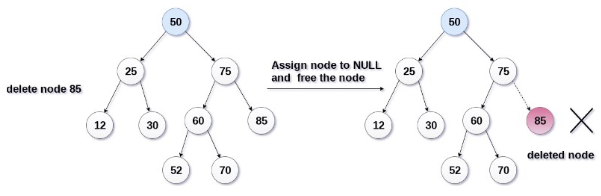
\includegraphics[width=0.8\textwidth]{image/Cancellazione1.png} \\ \\
        \end{tabular}
    \end{center}
    \item Il nodo da eliminare ha un solo figlio: si sostituisce il nodo con il suo nodofiglio e si elimina il nodo figlio, che ora contiene il valore da eliminare. È sufficiente sostituirlo con NULL e liberare lo spazio allocato. \\~\\
    Nell'immagine seguente, il nodo $12$ deve essere eliminato. Ha solo un figlio. Il nodo verrà sostituito con il suo nodo figlio e il nodo $12$ sostituito (che ora è un nodo foglia) verrà semplicemente eliminato.
    \begin{center}
        \begin{tabular}{c}
            \\ 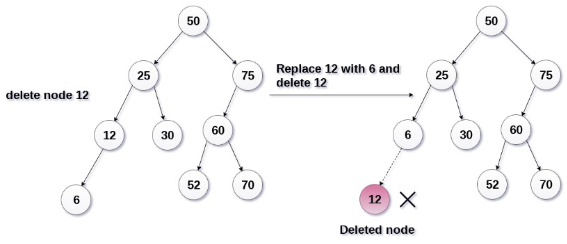
\includegraphics[width=0.65\textwidth]{image/Cancellazione2.png} \\ \\
        \end{tabular}
    \end{center}
    \item Il nodo che deve essere cancellato ha due nodi figli: il nodo da eliminare viene sostituito con il suo successore o predecessore in ordine ricorsivo, finché il valore del nodo (da eliminare) non viene collocato sulla foglia dell'albero. Al termine della procedura, si sostituisce il nodo con NULL e si libera lo spazio allocato. \\~\\
    Nell'immagine seguente, il nodo da eliminare è il nodo $50$, che è il nodo radice dell'albero. L'attraversamento in ordine sparso dell'albero: $6, 25, 30, 50, 52, 60, 70, 75$. Sostituire $50$ con il suo successore in ordine $52$. Ora $50$ verrà spostato alla foglia dell'albero, che verrà semplicemente eliminata.
    \begin{center}
        \begin{tabular}{c}
            \\ 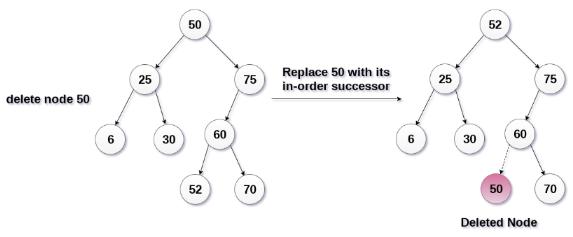
\includegraphics[width=0.65\textwidth]{image/Cancellazione3.png} \\ \\
        \end{tabular}
    \end{center}
\end{itemize}

\begin{mdframed}
\begin{lstlisting}[language=C]
DELETE(T,z)
1   if z.left == NULL
2       TRANSPLANT(T,z,z.right)
3   else if z.right == NULL
4       TRANSPLANT(T,z,z.left)
5   else
6       y = MIN(z.right)
7       if y.p != z
8           TRANSPLANT(T,y,y.right)
9           y.right = z.right
10          y.right.p = y
11      y.left = z.left
12      y.left.p = y
13      TRANSPLANT(T,z,y)
\end{lstlisting}
\end{mdframed}
Complessità: $O(h)$ \\~\\
Attenzione se dobbiamo esaminare tutto l'albero, nel caso peggiore avremo una complessità $\Theta(n)$ sulla base di una relazione di ricorrenza $T(n) = c + T(k) + T(n-k-1)$.

\newpage
